\section{Product Perspective}
The product is an open source, community driven service which is licensed under the GNU general Public
License. Product Aim is to provide an app offering a complete, rich and innovative feature set. User don't
have to suffer through any enraging registration. They can login using their college ID and password and
start using the service.\\
\noindent This service mainly is an implementation of client-server model. Where clients are: -
\begin{itemize}
\item Android application dedicated to college centric social network.
\item Web client enable non-android users to interact and enjoy the services.
\end{itemize}
\noindent And server is Ejabberd.\\
\noindent Ejabberd is an XMPP application server, written mainly in the Erlang programming language. It can run
under several Unix-like operating systems such as Mac OS X, GNU/Linux, FreeBSD, NetBSD, OpenBSD
and OpenSolaris.\\
\noindent Extensible Messaging and Presence Protocol (XMPP) is a communications protocol for message- oriented
middleware based on XML (Extensible Markup Language). It enables the near-real-time exchange of
structured yet extensible data between any two or more network entities. WhatsApp user the same server
and protocol to provide their services.
\section{Product Functions}
The system performs the following functions. The functions depend on the user’s level and permission
package, as explained in the user characteristics. Features that this project going to provide:
\begin{itemize}
\item Login with user ID or roll number.
\item Automatic conversation back up on the server, sparing your precious phone storage.
\item Save your contacts on your phone and / or with your account and port them to any phone via login.
\item Chat using multiple accounts from a single copy of the App.
\item End-to-end encryption with OMEMO.
\item Send and receive images as well as other kind of files.
\item Indication when your contact has read your message.
\item Pre-configured classification into groups for conference chats.
\end{itemize}
\section{User Characteristics}
Users of this project are the staff and students of the college. We can classify the users in the following
categories: -
\begin{itemize}
\item Students: Users who use the application on daily basis.
\item Teachers: They can use this app to interact with the students and ask queries to the chatbot.
\item College Authorities: Authorities can use the application to provide updates to students about the
various activities going in the college.
\end{itemize}
Also, the project is open source so there will be developers that contributes to the project in the future. They
can be students or teachers associated to develop the application.
\section{Constraints}
The software has the following constraints:
\begin{itemize}
\item Bad internet connectivity.
\item Server Traffic or any type of DDOS (Denial of Service) attack.
\item Flaw in database design
\item The project completed in the duration of 2 months.
\end{itemize}
\section{Data Flow Diagram}
A data flow diagram (DFD) maps out the flow of information for any process or system. It uses defined symbols like rectangles, circles and arrows, plus short text labels, to show data inputs, outputs, storage points and the routes between each destination
\begin{figure}[ht]
\centering
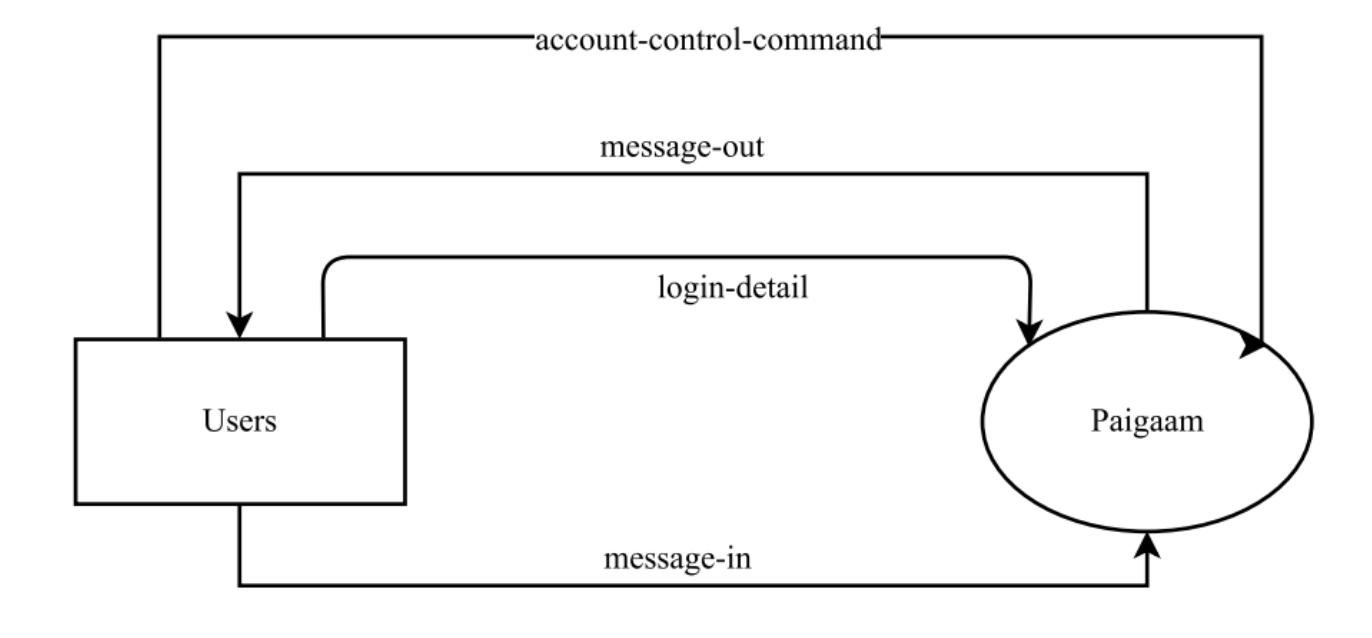
\includegraphics[scale=0.2]{input/images/dfd01.png}
\caption{Level 0 DFD}
\end{figure}
\begin{figure}[ht]
\centering
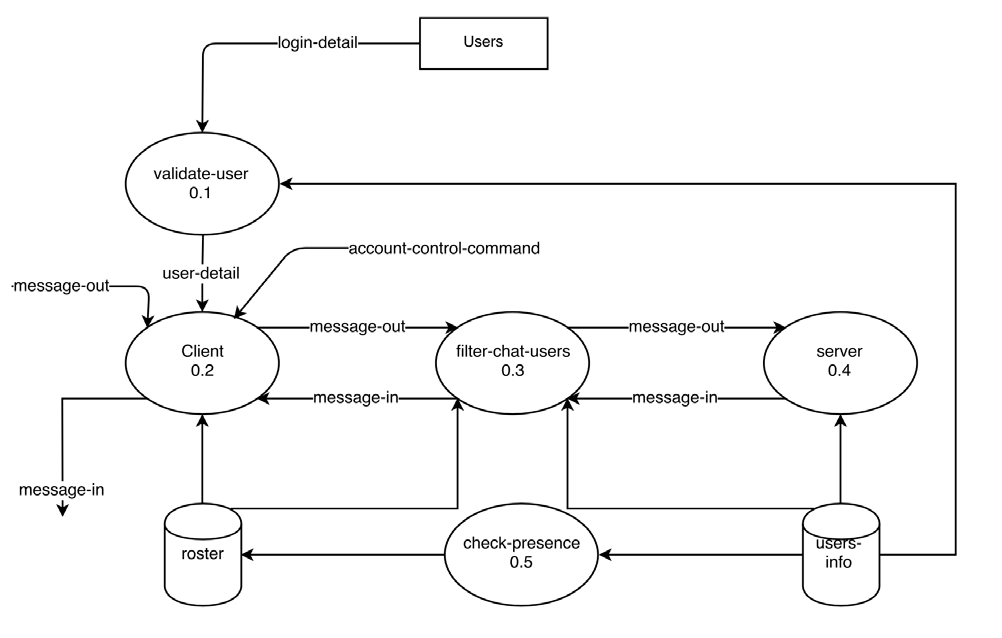
\includegraphics[scale=0.25]{input/images/dfd02.png}
\caption{Level 1 DFD}
\end{figure}
\newpage
\section{Flowchart}
A flowchart is a type of diagram that represents an algorithm, work flow or process, showing the steps as boxes of various kinds, and their order by connecting them with arrows.Each step in the sequence is noted within a diagram shape. Steps are linked by connecting lines and directional arrows.Today, flowcharts are used for a variety of purposes in manufacturing, architecture, engineering, business, technology, education, science, medicine, government, administration and many other disciplines. This allows anyone to view the flowchart and logically follow the process from beginning to end and following are flowchart of DoS showing flow of control and Data in the software-:
\begin{figure}[ht]
\centering
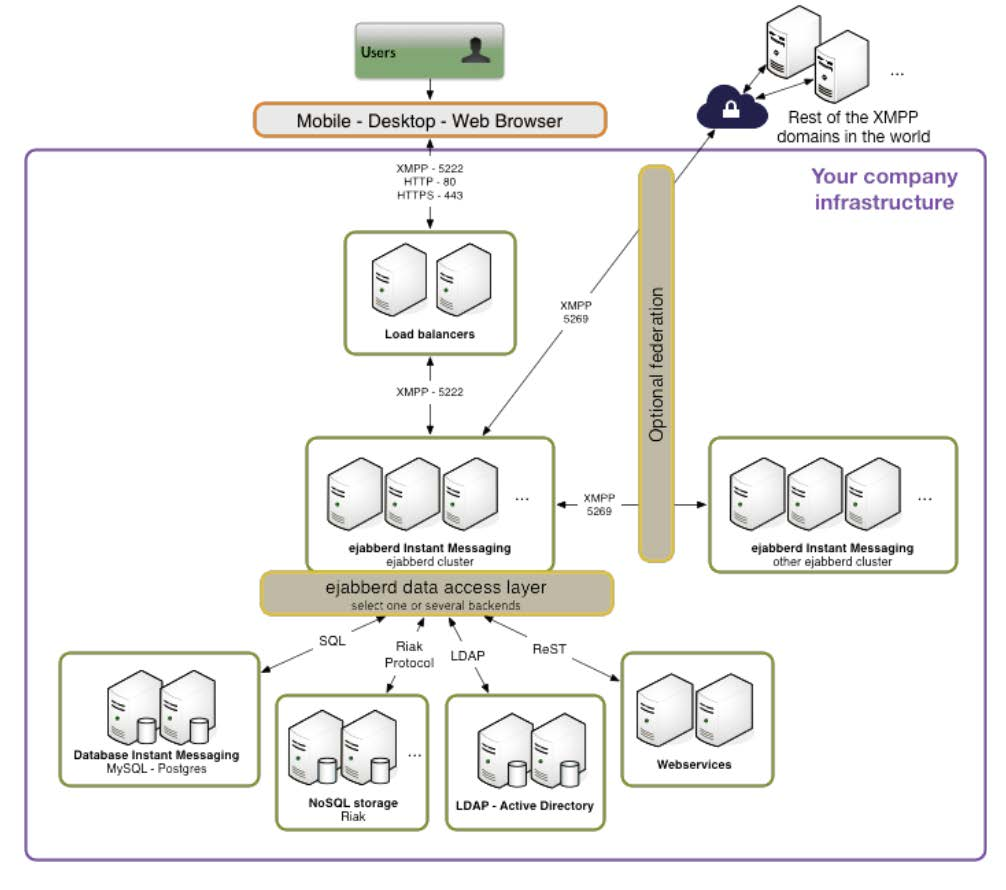
\includegraphics[scale=0.32]{input/images/fl.png}
\caption{Flow Chart}
\end{figure}
\hspace{-1.7em}
\newpage


\section{Table Structure}
\subsection{Paigaam}
Ejabberd SQL database schema is design in order to maintain all the record about the users and messages.\\

\noindent \textbf{Table users}\\
\noindent Contains the information required to authenticate users. 
\begin{figure}[ht]
\centering
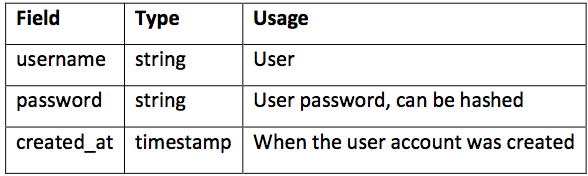
\includegraphics[scale=0.5]{input/images/t1.png}
\caption{Registered Users}
\end{figure}\\
\textbf{Table roster users}\\
\noindent This is a quite complex table, used as a store for a quite complex protocol that is the one defined to manage
rosters (groups) and subscriptions. In the common case of two users adding each other as contacts, entries
in the roster table follows a series of steps as they move from a subscription request to the final approval
and bi-directional subscription being established. This process can be initiated either by the user, or by the
(possible remote) peer.\\
\begin{figure}[ht]
\centering
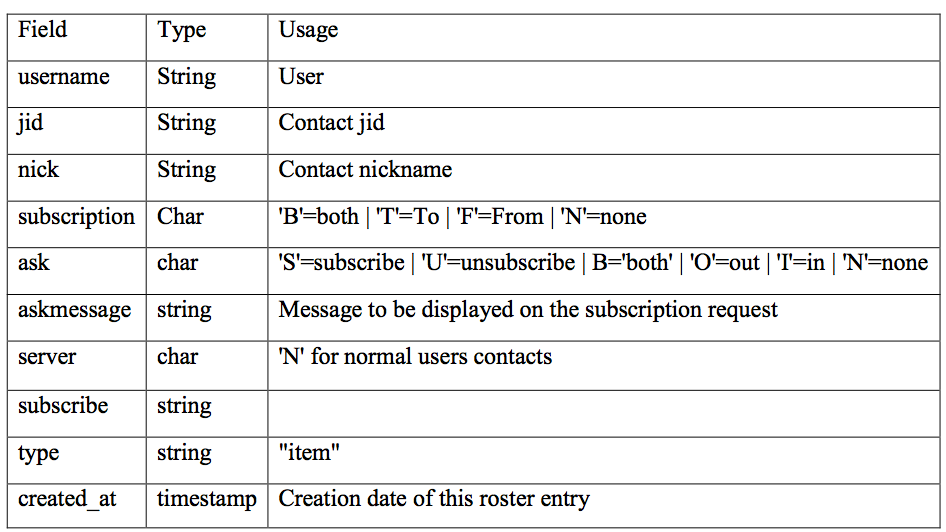
\includegraphics[scale=0.4]{input/images/t2.png}
\caption{Users in a Group}
\end{figure}\\
\noindent \textbf{Table spool}\\
\noindent Messages sent to users that are offline are stored in this table. Do not confuse this with general message
archiving: messages are only temporarily stored in this table, removed as soon as the target user is back
online and the pending messages delivered to it.\\
\begin{figure}[ht]
\centering
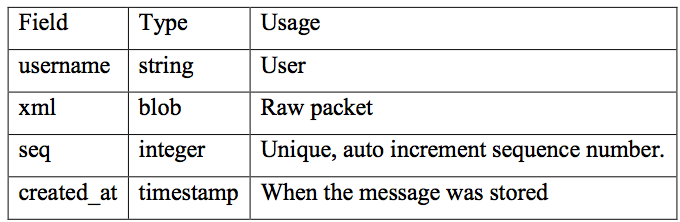
\includegraphics[scale=0.5]{input/images/t3.png}
\caption{Pending Messages}
\end{figure}\\
\textbf{Table privacy\_list\_data}\\
\noindent The table is used to store privacy rules.
\begin{figure}[ht]
\centering
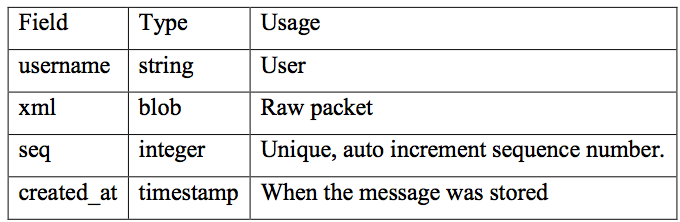
\includegraphics[scale=0.5]{input/images/t3.png}
\caption{Privacy Settings defined By User}
\end{figure}\\
\noindent \textbf{Table muc\_room}\\
\noindent It is used to store persistent rooms, that is, rooms that must be automatically started with the server.\\
\begin{figure}[ht]
\centering
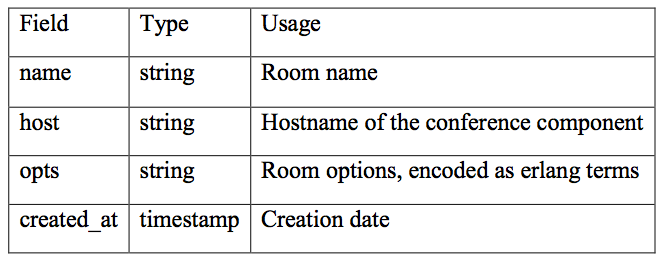
\includegraphics[scale=0.5]{input/images/t5.png}
\caption{Created Groups}
\end{figure}\\
\noindent \textbf{Table last}\\
\noindent This table is used to store the last time the user was seen online.\\
\begin{figure}[ht]
\centering
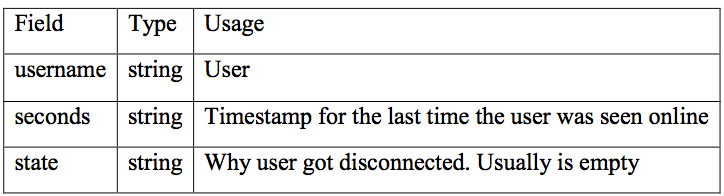
\includegraphics[scale=0.5]{input/images/t6.png}
\caption{Last Seen Information}
\end{figure}
\subsection{Chatbot(Paigaam-Assistant)}
\noindent \textbf{Table student\_details}\\
\noindent This table is used to store student details.\\
\begin{figure}[ht]
\centering
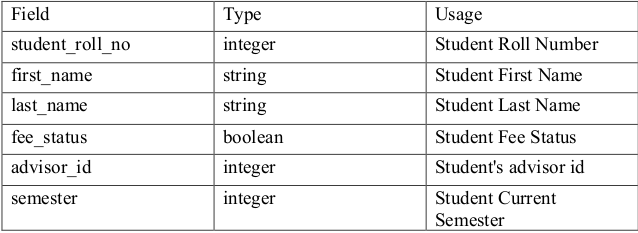
\includegraphics[scale=0.5]{input/images/t7.png}
\caption{Student Details}
\end{figure}\\\newpage
\noindent \textbf{Table Teacher Details	}\\
\noindent This table stores the details of teachers..\\
\begin{figure}[ht]
\centering
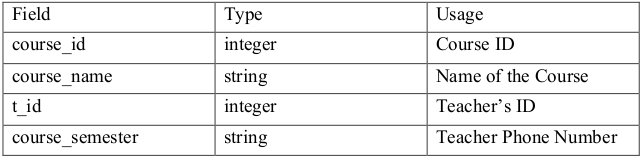
\includegraphics[scale=0.5]{input/images/t9.png}
\caption{Course Details}
\end{figure}\newpage
\section{ER Diagrams}
\begin{figure}[ht]
\centering
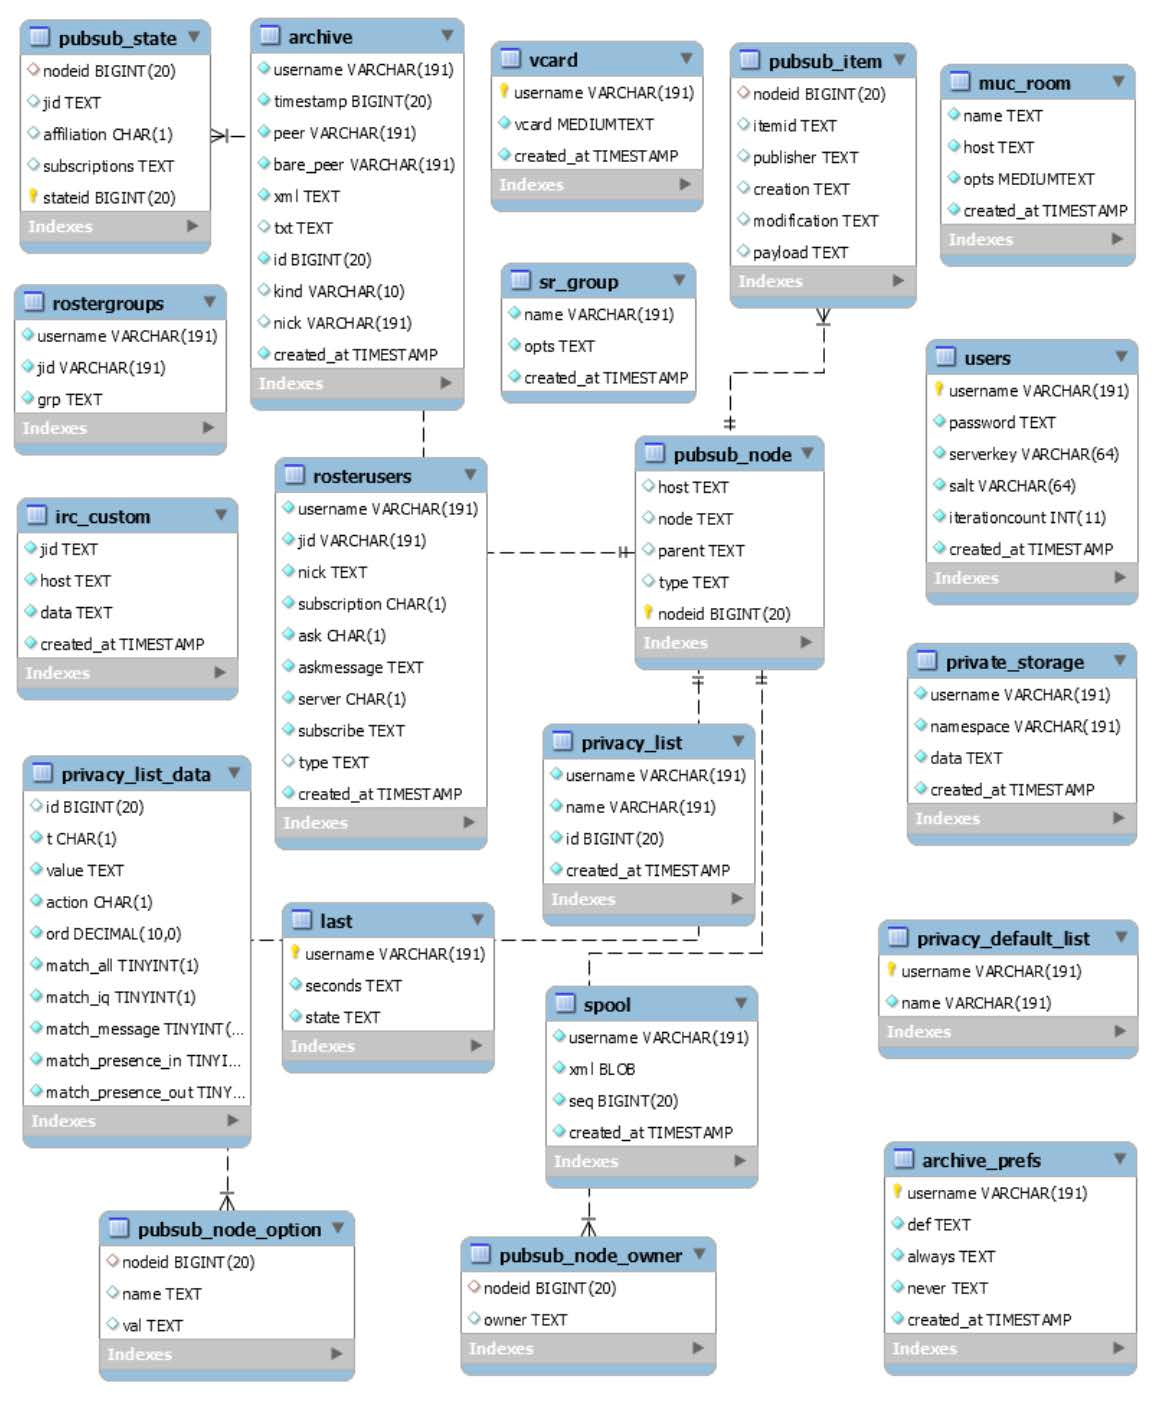
\includegraphics[scale=0.35]{input/images/er1.png}
\caption{Paigaam ER Diagram}
\end{figure}
\newpage
\begin{figure}[ht]
\centering
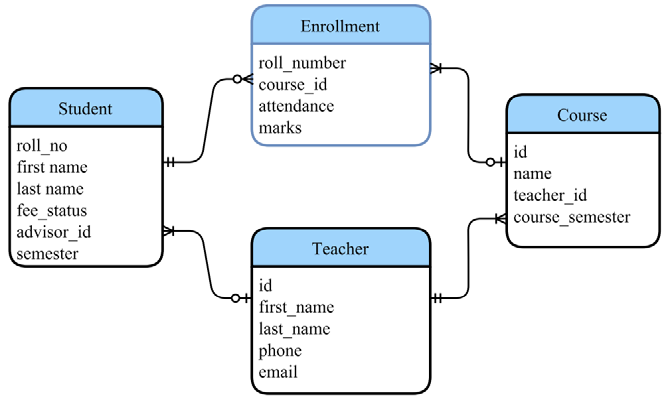
\includegraphics[scale=0.3]{input/images/erp.png}
\caption{Paigaam ER Diagram}
\end{figure}
\subsection{Assumptions and Dependencies}
This system is provisioned to be built on the Android Platform which is highly flexible. Decision regarding
which database to use should be taken considering the fact that data being exchanged or stored is large, and
the appropriate data management system will yield efficient performance.
The software has the following dependencies:
\begin{itemize}
\item The system is highly dependent on internet connectivity and required permissions to send/receive
the messages to/from the server.
\item Android operating system should be updated to at least 4.0 version.
\end{itemize}
\subsection{Specific Requirements}
\subsubsection{Software Requirements}
For developing the application, the following are the Software Requirements:
\begin{itemize}
\item Operating System: Windows 10, Android 4.0 KitKat, Linux
\item Languages: HTML, CSS, JavaScript \& Python, Java.
\item Database: SQLite.
\item Tools: Web Browser: Chrome, Firefox, Sleek XMPP, Errbot.
\end{itemize}
\subsubsection{Hardware Requirements}
For developing the application, the following are the Hardware Requirements:
\begin{itemize}
\item Processor: Intel core i3.
\item RAM: 4GB.
\end{itemize}

%\section{Types of Feasibility Study}
%\noindent Feasibility analysis involved a thorough assessment of the operational and technical aspects of the proposal.
%Feasibility study tested the system proposal and identified whether the user needs may be satisfied using
%the current software and hardware technologies, whether the system will be cost effective from a business
%point of view and whether it can be developed with the most up to date technologies.
%\subsection{Operational Feasibility}
%\noindent Operational feasibility is a measure of how well a project solves the problems, and takes advantage of
%the opportunities identified during scope definition and how it satisfies the requirements identified in
%the requirements analysis phase of system development. All the operations performed in the software
%are very quick and satisfy all the requirements.
%\subsection{Technical Feasibility}
%\noindent Technological feasibility is carried out to determine whether the project has the capability, in terms
%of software, hardware, personnel to handle and fulfill the user requirements. The assessment is based
%on an outline design of system requirements in terms of Input, Processes, Output and Procedures.
%OpenStreetMap is technically feasible as it is built up using various open source technologies and it can run on any platform.
%\subsection{Economic Feasibility}
%\noindent Economic analysis is the most frequently used method to determine the cost/benefit factor for evalu-
%ating the effectiveness of a new system. In this analysis we determine whether the benefit is gained
%according to the cost invested to develop the project or not. If benefits outweigh costs, only then
%the decision is made to design and implement the system. It is important to identify cost and benefit
%factors, which can be categorized as follows:
%\begin{itemize}
%\item Development Cost
%\item Operation Cost
%\end{itemize}
%This System is Economically feasible with 0 Development and Operating Charges
%as it is developed in Qt Framework and libdxfrw library which is open source technology and is available free of cost on the internet.
